\documentclass[12pt,a4paper]{article} 
\usepackage[portuguese]{babel} \usepackage[utf8]{inputenc}
\usepackage{amsmath} 
\usepackage{graphicx}
\usepackage{booktabs}
\usepackage{float}
\begin{document}
\setcounter{figure}{2}
\setcounter{section}{3}
\setcounter{page}{5}
\section{Relatório}
\subsection{Introdução}

Nesta prática, deseja-se entender o funcionamento básico de um transistor de junção bipolar, através de análises em DC e AC. 

Um transistor de junção bipolar é um transistor que usa tanto lacunas e elétrons como portadores de cargas, 
em contraste com os transistores unipolares, como o MOSFET, que apenas utiliza um tipo de portador de carga para sua operação. 

A operação de um transistor bipolar de junção vem de duas junções entre dois tipos de semicondutores, tipo \emph{n} e tipo \emph{p}. 
Desta forma existem dois tipos de \emph{TBJ}; \emph{PNP} e \emph{NPN}.  Os estados destas duas junções, junção emissor-base (EBJ) e
junção coletor-base (CBJ) definem o comportamento do transistor, se ele está em saturação, corte ou ativo, conforme a Tabela~\ref{tab:operacao}  %Insirir ref aqui
nos mostra.  

\begin{table}[htpb]
  \centering
  \caption{Tabela de modos de operação do transitor TBJ. }
  \label{tab:operacao}
  \begin{tabular}{c c c}
    \toprule  \\
    Modo       & EBJ                    & CBJ                    \\ \midrule
    Corte      & Reverso                & Reverso                \\ \midrule
    Ativo      & Diretamente polarizado & Reverso                \\ \midrule
    Saturação  & Diretamente polarizado & Diretamente polarizado \\ \bottomrule
  \end{tabular}
\end{table}

Este tipo de transistor é largamente utilizado para amplificação de corrente e utilizado como chave em uma vasta gama de aplicações 
na in eletrônica. O transistor bipolar em aplicações de amplificação normalmente funciona no modo ativo enquanto
quando funciona como uma chave pode ser utilizado tanto em saturação quanto no modo ativo.

\begin{figure}[htpb]
  \centering
  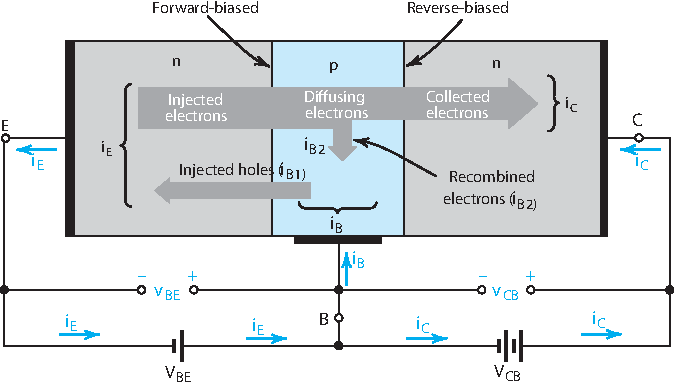
\includegraphics[width=0.8\linewidth]{img/bjt_current.pdf}
  \caption{Corrente fluindo em um transistor npn polarizado para operar no modo ativo.}
  \label{fig:bjt_current}
\end{figure}

O transistor \emph{BJT} \emph{NPN} em modo ativo requer uma tensão $V_{BE}$ aplicada de forma
que a base tipo \emph{P} esteja a um potencial maior que o emissor de tipo \emph{N}, logo deixando
a junção \emph{EBJ} diretamente polarizada. A junção \emph{CBJ}, no entanto, precisa estar 
polarizada reversamente e para isso o coletor de tipo \emph{N} precisa estar a um potencial maior 
que a base tipo \emph{P}. \\
Como a junção \emph{EBJ} está diretamente polarizada, uma corrente fluirá. Corrente composta por 
dois componentes: elétrons injetados do emissor na base e lacunas injetadas da base no emissor. 
A corrente no coletor será proporcional a $e^{\frac{v_{BE}}{v_{T}}}$ é dada por:
\begin{align*}
  i_c = I_{s}e^{\frac{v_{BE}}{V_{T}}}
\end{align*}
E a corrente na base:
\begin{align*}
  i_b = \frac{I_s}{\beta} e^{\frac{v_{BE}}{V_{T}}}
\end{align*}
E no emissor:
\begin{align*}
  i_e = \frac{\beta +1}{\beta}  i_c
\end{align*}

\subsection{Análises}
\begin{figure}[htpb]
  \centering
  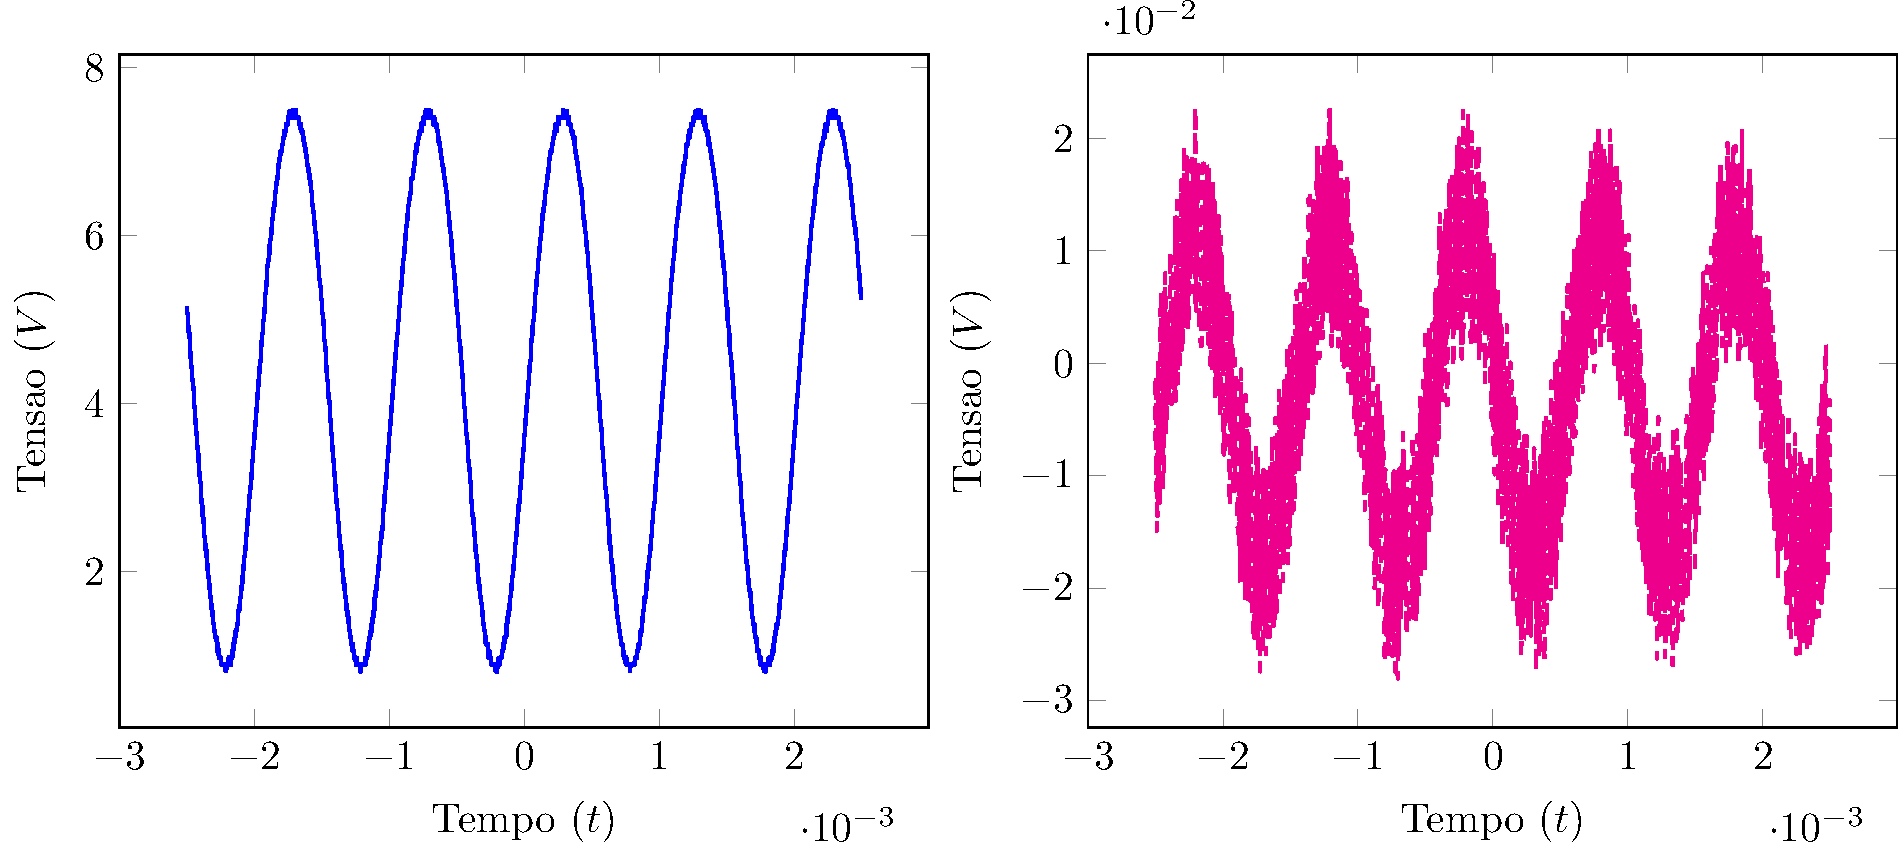
\includegraphics[width=0.8\linewidth]{img/scope_1.pdf}
  \caption{Sinal senoidal de frequência 1\emph{KHz} aplicada a entrada do circuito da Figura~1, representado na cor magenta, e sua respectiva saída representada em azul.}
  \label{fig:1khz}
\end{figure}
\begin{figure}[htpb]
  \centering
  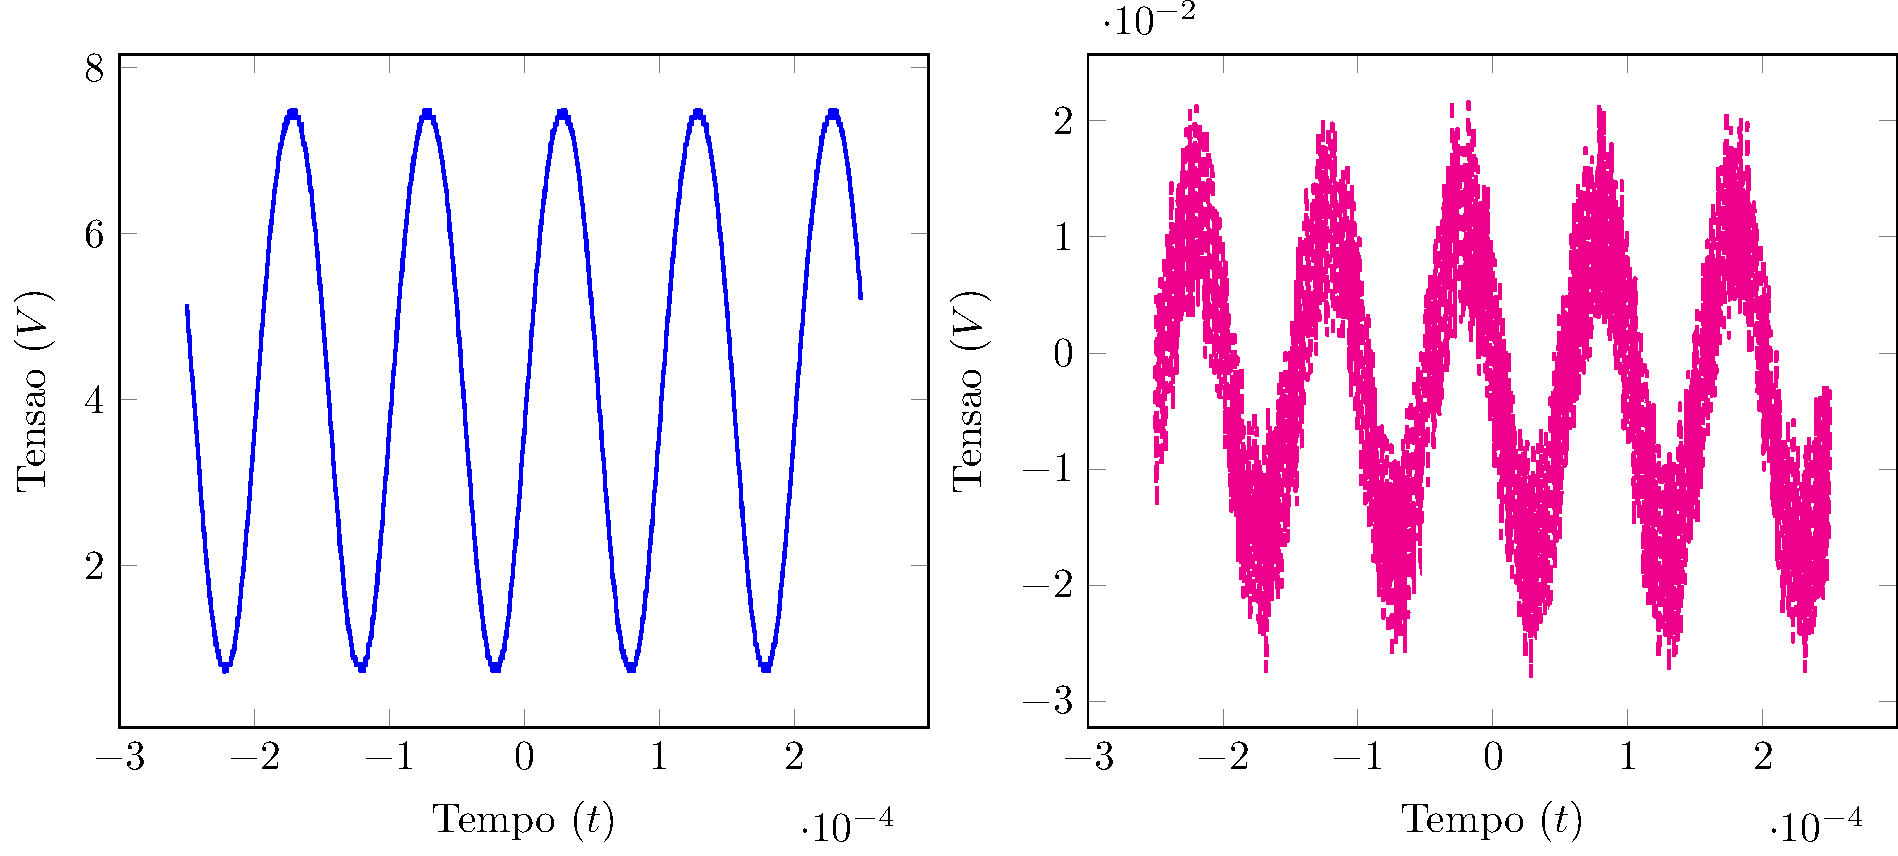
\includegraphics[width=0.8\linewidth]{img/scope_2.pdf}
  \caption{Sinal senoidal de frequência 10\emph{KHz} aplicada a entrada do circuito da Figura~1, representado na cor magenta, e sua respectiva saída representada em azul.}
  \label{fig:10khz}
\end{figure}
\begin{figure}[htpb]
  \centering
  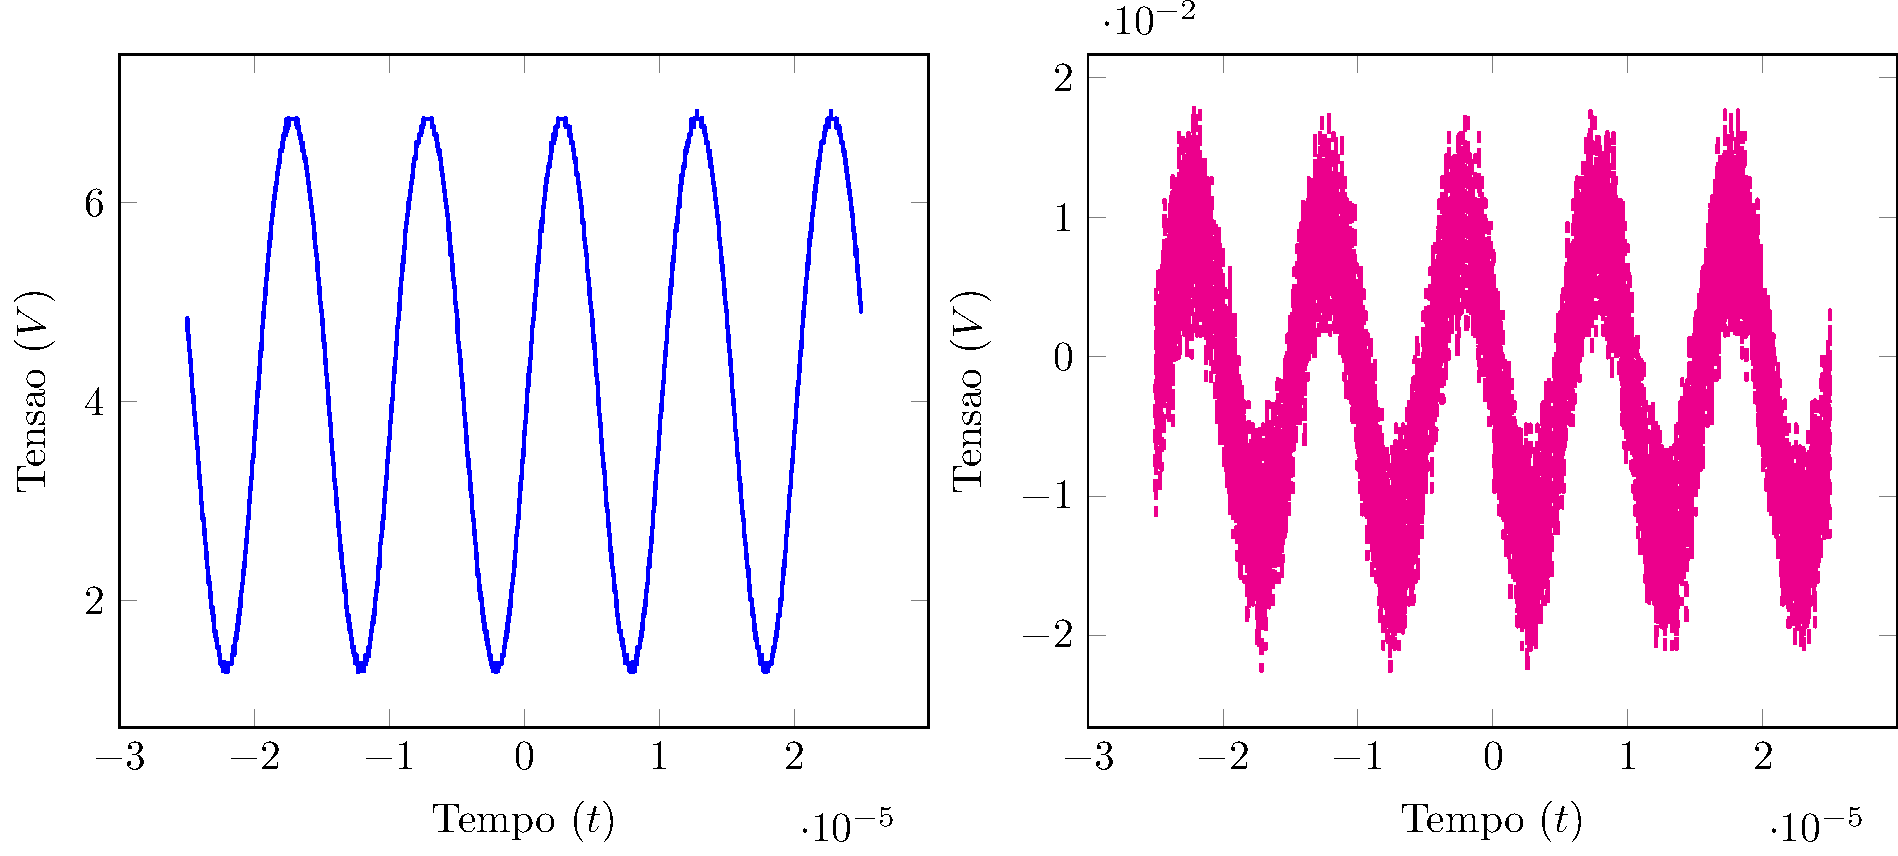
\includegraphics[width=0.8\linewidth]{img/scope_5.pdf}
  \caption{Sinal senoidal de frequência 100\emph{KHz} aplicada a entrada do circuito da Figura~1, representado na cor magenta, e sua respectiva saída representada em azul.}
  \label{fig:100khz}
\end{figure}


\begin{table}[htpb]
  \centering
  \caption{Parâmetros de vários transistores bipolares da mesma do circuito em DC.}
  \label{tab:expdc}
  \begin{tabular}{c c c}
    \toprule
    $I_{BQ} [\mu A]$ & $I_{CQ}[mA]$ & $V_{CEQ}[V]$ \\ \midrule
    51               & 14.2         & 5.43         \\ \midrule
    51               & 14           & 4.8          \\ \midrule
    51               & 16           & 4.07         \\ \bottomrule
  \end{tabular}
\end{table}
\begin{table}[htpb]
  \centering
  \caption{Tabela de ganho para diferentes frequências do sinal de entrada.}
  \label{tab:osci}
  \begin{tabular}{c c c c}
    \toprule   
    Frequência  & Entrada  CA RMS [$mV$] & Saída CA RMS [V] & Ganho  \\ \midrule
    1KHz        & 11.52                  & 2.34             & -203   \\ \midrule
    10KHz       & 11.17                  & 2.39             & -213.9 \\ \midrule
    100KHz      & 10.32                  & 1.958            & -189.7 \\ \bottomrule
  \end{tabular}
\end{table}

\newpage
\subsection{Discussões}
A Tabela~\ref{tab:expdc} se refere a dados coletados de três transistores da família
BC237. Esperávamos, pela teoria, que $I_{BQ}$ fosse $50\mu A$, o que foi confirmado 
pelos dados empíricos, assim como $I_{CQ}$ que deveria estar na faixa de $10 mA$ 
mas variou entre $14.2$ e $16$ miliampéres.No entanto, o $V_{CEQ}$ tiveram resultados
bem diferentes do esperado, de $8V$ esperado obtivemos valores numa faixa de $4$ a $6V$.

Os ganhos para os transistores foram de $313$, $274$ e $278$. Percebe-se que existe 
uma variância relativamente grande entre eles e que o ganho teórico de 200 foi um 
resultado subestimado.


Para o experimento dois, podemos analisar o ganho medido no osciloscópio através da 
Tabela~\ref{tab:osci}. Em uma análise teórica, poderíamos considerar o capacitor na entrada
suficientemente grande e a partir do modelo de pequenos sinais, estimar o ganho teórico.
Esta análise nos resultaria na relação abaixo (o valor medido do transistor $R_{c}$ é $676\Omega$):
\begin{align*}
  \frac{V_{c}}{V_{in}}  = -g_{m} \times R_{c}=  -\frac{10mA}{25mV} \times 676 \Omega = -270
\end{align*}

O que segundo a Tabela~\ref{tab:osci} não aparenta ser um resultado razoável, já que 
existe uma diferença grande entre a teoria e os resultados práticos. Isso pode ser 
relacionado com o fato de o modelo de pequenos sinais ser uma boa aproximação apenas 
para variações de amplitude menores que $10mV$ o que , no caso, não foi devidamente respeitado
pelos sinais de entrada.
\newpage
\subsection{Conclusão}
Nesta prática foram abordados conceitos a cerca do funcionamento de um transistor bipolar de junção, 
como testá-lo com um multímetro, qual deve ser o dimensionamento dos componentes do circuito para 
o funcionamento correto do transistor e quais as condições de operação do mesmo.

Recalculou-se através das resistências reais, os valores reais da corrente do circuito do transistor e,
depois de validada, comparou-se com os resultados teóricos. Mediu-se também os valores
da corrente da base, corrente do coletor e tensão coletor-base, que possibilitou
calcular o ganho dos três transistores. Concluimos então que o 
ganho dos transistores se apresentou maior que na teoria que, em um análise conservativa, 
subestimou o ganho real.

O segundo experimento, envolveu análise em AC, com um sinal de entrada senoidal aplicado 
em diversas frequências. Um osciloscópio capturou os sinais de entrada e saída para os casos
de 1kHZ, 10kHz e 10kHZ que possibilitaram entender como o sinal amplificado é. O ganho 
teórico foi calculado então e comparado com o sinal real. Estes ganhos se provaram bem 
diferentes, provavelmente pela condição de validade do modelo de pequenos sinais utilizado.

Desta forma, pôde-se entender o funcionamento básico de um transistor bipolar tanto em DC 
quanto em AC.
\end{document}
